% Template for Cogsci submission with R Markdown

% Stuff changed from original Markdown PLOS Template
\documentclass[10pt, letterpaper]{article}

\usepackage{cogsci}
\usepackage{pslatex}
\usepackage{float}
\usepackage{caption}

% amsmath package, useful for mathematical formulas
\usepackage{amsmath}

% amssymb package, useful for mathematical symbols
\usepackage{amssymb}

% hyperref package, useful for hyperlinks
\usepackage{hyperref}

% graphicx package, useful for including eps and pdf graphics
% include graphics with the command \includegraphics
\usepackage{graphicx}

% Sweave(-like)
\usepackage{fancyvrb}
\DefineVerbatimEnvironment{Sinput}{Verbatim}{fontshape=sl}
\DefineVerbatimEnvironment{Soutput}{Verbatim}{}
\DefineVerbatimEnvironment{Scode}{Verbatim}{fontshape=sl}
\newenvironment{Schunk}{}{}
\DefineVerbatimEnvironment{Code}{Verbatim}{}
\DefineVerbatimEnvironment{CodeInput}{Verbatim}{fontshape=sl}
\DefineVerbatimEnvironment{CodeOutput}{Verbatim}{}
\newenvironment{CodeChunk}{}{}

% cite package, to clean up citations in the main text. Do not remove.
\usepackage{apacite}

% KM added 1/4/18 to allow control of blind submission


\usepackage{color}

% Use doublespacing - comment out for single spacing
%\usepackage{setspace}
%\doublespacing


% % Text layout
% \topmargin 0.0cm
% \oddsidemargin 0.5cm
% \evensidemargin 0.5cm
% \textwidth 16cm
% \textheight 21cm

\title{Characterizing the object categories two children see and interact with
in a dense dataset of naturalistic visual experience}


\author{}

\begin{document}

\maketitle

\begin{abstract}
What do infants and young children tend to see in their everyday lives?
Relatively little work has examined the categories and objects that tend
to be in the infant view during everyday experience, despite the fact
that this knowledge is central to theories of category learning. Here,
we analyzed the prevalence of the categories (e.g., people, animals,
food) in the infant view in a longitudinal dataset of egocentric infant
visual experience. Overall, we found a surprising amount of consistency
in the broad characteristics of children's visual environment across
individuals and across developmental time, in contrast to prior work
examining the changing nature of the social signals in the infant view.
In addition, we analyzed the distribution and identity of the categories
that children tended touch and interact with in this dataset,
generalizing previous findings that these objects tended to be
distributed in a Zipfian manner. Taken together, these findings take a
first step towards characterizing infants' changing visual environment,
and call for future work to examine the generalizability of these
results and to link them to learning outcomes.

\textbf{Keywords:}
Object categorization; infant visual experience; head-mounted cameras;
longitudinal data.
\end{abstract}

\hypertarget{introduction}{%
\section{Introduction}\label{introduction}}

What do children tend to see in their everyday lives? While an
understanding of children's visual environment is central to both
theories of language acquisition and visual development, we know
remarkably little about the categories and objects that tend to be in
the infant view, or in what format they are experienced. For example,
how often do infants tend to see animals in real-life vs.~in storybooks
or as toys? How consistent are children's visual environments across
individuals and across developmental time?

Over the past decade, researchers have begun to answer these questions
by documenting the infant egocentric perspective using head-mounted
cameras (Franchak, Kretch, Soska, \& Adolph, 2011; Yoshida \& Smith,
2008) and quantifying the degree to which there are substantial shifts
in infants' viewpoints that may have downstream developmental
consequences. As adults, it is hard to intuit how strange this viewpoint
can be, and how much it varies across development, transitioning over
the first two years of life from close-up views of faces to restricted
views of hands manipulating objects (Fausey, Jayaraman, \& Smith, 2016;
Long, Kachergis, Agrawal, \& Frank, 2020), with children's postural
developments to a large extent shaping what they see (Sanchez, Long,
Kraus, \& Frank, 2018). Most work, however, has focused on documenting
the social information that infants and children have access to across
early development (Fausey et al., 2016; Sanchez et al., 2018; Yoshida \&
Smith, 2008).

\begin{CodeChunk}
\begin{figure*}[h]

{\centering 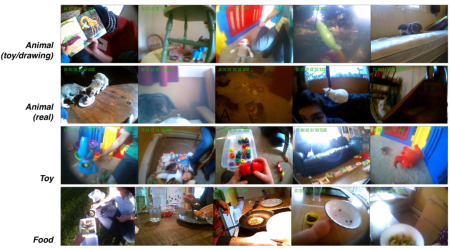
\includegraphics{figs/examples-1} 

}

\caption[Example frames with annotations of four different categories]{Example frames with annotations of four different categories.}\label{fig:examples}
\end{figure*}
\end{CodeChunk}

More recent research has made progress towards understanding what
objects tend to be the infant view, starting with analyzing the
basic-level categories (e.g., spoons, cups) in the view of 8-month-olds
during mealtime. This work suggests that a small number of objects are
both pervasively present during mealtime and among infants'
first-learned words (Clerkin, Hart, Rehg, Yu, \& Smith, 2017), pointing
towards a link between visual experience and early word learning and
category learning.

Thus, a more complete understanding of the visual environment of infants
and young children could yield insights about the inputs to both
category learning and word learning. Indeed, different distributions of
these visual referents lead to constraints on the kinds of learning
mechanisms that must operate to form robust category representations --
and to learn words for these categories. However, at present, no
datasets are sufficiently annotated to constrain these theoretical
accounts.

For example, if the categories in the infant view shift dramatically
over the first few years of life, then we might expect infants to learn
about certain categories earlier vs.~later during development. Prior
work documenting the proportion of social information in view has
suggested that children see more hands relative to faces in this same
age range (Fausey et al., 2016; Long et al., 2020). Thus, one
possibility is that as children learn to crawl and walk (Franchak et
al., 2011; Long et al., 2020; Sanchez et al., 2018), categories that
children are likely to interact with (i.e., toys, small objects) may
also become more prevalent in the child's view. If this was the case,
this finding would support a view where the inputs to early category
learning are shaped by children's own ability to actively explore their
environment.

On the other hand, the broad characteristics of children's visual
environments may be relatively stable and mostly determined by the
activities that they tend to engage in. Indeed, some theoretical
accounts have suggested that the statistics of children's visual
environment are mostly driven by these stereotyped activity contexts
(Bruner, 1985) -- e.g.~mealtime or storytime -- and that children learn
most robustly in these contexts. On these accounts, children might
become very sensitive to the co-occurrences between different activities
(e.g., eating) and object categories (e.g., spoons, food). However, no
work has identified how consistently categories co-occur in natural
environments. For example, while some activity contexts (e.g.,
storytime) lead to intuitive co-occurrences between object categories
(e.g., between books and people), not all activity contexts will
generate intuitive or consistent co-occurrences between object
categories.

Finally, \emph{how} infants interact with object categories will
undoubtedly change what they learn about them. For example, children
tend to generate informative views of objects while manipulating them --
and, early in development, children's ability to sit and manipulate
objects correlates with their perceptual abilities (Soska, Adolph, \&
Johnson, 2010). Yet while most datasets used to train deep neural
network models contain only photographs of object categories, many
children -- especially those in Western, industrialized cultures -- will
likely experience many categories through picture books as flat,
stylized, 2D depictions. If children see very few real-life exemplars of
a category relative to depictions (e.g., giraffes), this suggests that
children must learn to generalize between these different visual formats
in order to group these exemplars into one category. Further, this
implies that these representations might be coarser than those
experienced across many different formats. And if children only interact
and manipulate a few small set of categories -- as suggested by Clerkin
et al., 2017 -- children may first learn about these frequently
experienced categories and then use these representations to generalize
to the categories they encounter very infrequently.

Here, we take a step towards answering these questions by characterizing
the visual environment of two young children in a longitudinal corpus of
head-mounted camera data (Sullivan, Mei, Perfors, Wojcik, \& Frank,
2020) from 6-32 months of age. To characterize trends in the visual
environment over development, we collected annotations of several
categories of objects (e.g., \emph{animals}, \emph{vehicles},
\emph{toys}, \emph{food}, \emph{furniture}) present in the infant view,
obtaining annotations on a randomly sampled set of 24,000 frames
(i.e.~around 59 frames per hour of recorded video). To provide a closer
look into the kinds of objects children have the most intensive visual
and haptic experience with, we also examined the specific objects that
children interacted with during everyday activities. To do so, we
annotated the basic-level identities (e.g., \emph{spoon}, \emph{marker})
of the objects that children were interacting with in the subset of
frames where children's hands were visible.

\begin{CodeChunk}
\begin{figure*}[h]

{\centering \includegraphics{figs/freq_by_category-1} 

}

\caption[Frequency of categories annotated across the 24K random frames plotted as a function of each child's age (in months)]{Frequency of categories annotated across the 24K random frames plotted as a function of each child's age (in months); each child's age was calculated in days relative to the date that the videos were filmed and converted to months. Each color represents data from a different child.}\label{fig:freq_by_category}
\end{figure*}
\end{CodeChunk}

\hypertarget{method}{%
\section{Method}\label{method}}

\hypertarget{dataset}{%
\subsection{Dataset}\label{dataset}}

The dataset is described in detail in Sullivan et al. (2020). Children
wore Veho Muvi miniature cameras mounted on a custom camping headlamp
harness (``headcams'') at least twice weekly, for approximately one hour
per recording session. One weekly session was on the same day each week
at a roughly constant time of day, while the other(s) were chosen
arbitrarily at the participating family's discretion. At the time of the
recording, all three children were in single-child households. Videos
captured by the headcam were 640x480 pixels, and a fisheye lens was
attached to the camera to increase the field of view to approximately
109 degrees horizontal x 70 degrees vertical. We randomly sampled 24,000
frames from videos of two of the children in the dataset (S, A) over the
entire age range.

\hypertarget{annotation-procedures}{%
\subsection{Annotation procedures}\label{annotation-procedures}}

\hypertarget{categories-in-the-infant-view}{%
\subsubsection{Categories in the infant
view}\label{categories-in-the-infant-view}}

Annotations of the categories in the dataset were obtained using AWS
Sagemaker. Participants selected whether the following categories were
present in the shown image: \emph{Animal (real), Animal (toy/drawing),
Vehicle (real), Vehicle (toy/drawing), Plant, Clothing, Person,
Furniture, Food, Utensil/Dish, Other Small Object, Other Big Object,
Book, None of the above}, or \emph{Nothing visible}. We included
\emph{Other Small Object} and \emph{Other Big Object} as categories that
participants could use to indicate the presence of objects that fell
outside of these categories but were still salient; additional
instructions were provided to specify that \emph{Other Big Object}
refers to objects bigger than a chair, and that \emph{Other Small
Object} refers to objects small enough to be held with one or two hands
(Konkle \& Caramazza, 2013). Two participants annotated each image, and
were required to select at least one category before proceeding. Each
category annotation in each image was assigned a confidence score
(possible range: 0-1, range in dataset: 0.5-1) and individual
annotations that had confidence scores below the 25th percentile were
excluded from analyses (although all conclusions hold with and without
these low-confidence annotations).

\begin{CodeChunk}
\begin{figure*}[h]

{\centering \includegraphics{figs/anim_size-1} 

}

\caption[Frequency of animals (including toys) relative to big and small inanimate objects detected in the dataset, both when analyzing all frames that were annotated (left) and the subset of frames where a child's hand was visible in the frame (right)]{Frequency of animals (including toys) relative to big and small inanimate objects detected in the dataset, both when analyzing all frames that were annotated (left) and the subset of frames where a child's hand was visible in the frame (right).}\label{fig:anim_size}
\end{figure*}
\end{CodeChunk}

We assessed the reliability of these annotations by comparing them to
annotations made on the same task for a random subsample of 1200 frames
on AWS Sagemaker, again using two participants per image (\(N\)=950
frames after excluding low-confidence annotations). We found agreement
was moderate (average Cohen's Kappa = 0.29, but varied substantially
between different categories (range = 0.02, 0.59), as Cohen's Kappa is
known to be harsh for sparse annotations. On average, there was
disagreement rate of 11.41\% across categories. Annotators disagreed
most on whether \emph{Clothing} was present in an image and whether
\emph{Other Big Object} was present (i.e.~a big object that was not
\emph{Furniture} or a \emph{Vehicle}). To assess the nature of these
disagreements, we manually examined a random sample of 160 images with
disagreements with 10 images from each category. There were relatively
equal proportions of images where annotations failed to identify a clear
example of a category (M=25\%) or where annotations select an erroneous
category label (M=24\%). However, we found that most (M=50.62\%) of the
disagreements resulted from ambiguous exemplars, for example where the
category was present but very distant, occluded, or blurry. Annotators
also showed some disagreement about whether glossy photos of different
categories in books should be counted as ``real'' or ``toy/drawing,''
and whether partial views of people (i.e.~child's own hands) should
count as a \emph{Person}. Going forward, we analyze the larger set of
annotations with the caveat that there is inevitably some ambiguity in
what counts as an exemplar of these categories and that these data
include both misses and false alarms. All annotations and analysis code
are openly available at the anonymized repository associated with this
project
(\url{https://osf.io/ft4ka/?view_only=b7387c0ceff845b0923b5871dee60d05}).

\hypertarget{objects-children-interacted-with}{%
\subsubsection{Objects children interacted
with}\label{objects-children-interacted-with}}

We also annotated the objects that children were interacting with in a
subset of these frames. To do so, we first selected the frames in which
participants (recruited via Amazon Mechanical Turk) indicated that a
child's hand or hands were visible in the image (see Long et al., 2020)
and one author annotated 1817 of these frames, spanning 7 to 28 months
of age with roughly equal proportions from the two children. The
annotator noted what object the child was touching or pointing to with
in frames containing children's hands, using basic-level object
categories such as ``block'' and ``cracker.'' If a child was holding a
book and pointing to a depicted object in the book, the depicted object
was noted as the category they were interacting with; otherwise, it was
noted as \emph{Book}. Food that was unidentifiable as a specific item
(e.g., as crackers) was marked as ``food,'' and baby toys that were
unidentifiable as specific toys were marked ``toy.'' When children were
interacting with drawing or toy versions of different categories (e.g.,
a toy car), these annotations were marked with a `-drawing' and `-toy'
modifier and counted as separate entries. If a view was allocentric,
there were no child hands in view, or there were no objects that were
visible, these frames were excluded from analysis; this left 1313 frames
with annotations.

\hypertarget{results}{%
\section{Results}\label{results}}

\hypertarget{which-categories-are-prevalent-in-the-childs-view}{%
\subsection{Which categories are prevalent in the child's
view?}\label{which-categories-are-prevalent-in-the-childs-view}}

First, we examined the overall prevalence of each category in the infant
view. Somewhat surprisingly, we found that the prevalence of most of
these categories were relatively stable both across the two children in
the dataset as well as over developmental time (see Figure
\ref{fig:freq_by_category}). This stands in contrast to prior work on
the prevalence of faces/hands in the infant view (Fausey et al., 2016;
Long et al., 2020), suggesting that these broader characteristics of
children's visual experience may be more consistent.

We next examined the details of these environments. We found that people
were by far the most prevalent of these categories: over 20\%~of the
annotated frames contained people, far more than any other category
(including all kinds of toys combined). In contrast, there were
relatively few instances of animals in the infant view -- either as toys
or their real-life counterparts. Less than 5\%~of the frames contained
any kind of depicted or real animal, and those few frames that did
contained depicted vs.~real animals in equal proportion. Manual
inspection of these frames containing animals revealed that the ``real''
animals had relatively little variety -- they were overwhelmingly frames
containing images of household pets (i.e., cats, dogs, and chickens, in
the case of A), whereas the animals that were ``toys/drawings'' depicted
a much larger variety of animals, as one might expect. Overall, these
results suggest that -- at least for these children -- people are much
more frequent that depictions or real-life versions of animals,
indicating that toys and drawings may provide frequent input to their
representations of these categories -- despite the fact that animal
names are often among children's first words (Frank, Braginsky,
Yurovsky, \& Marchman, 2021) and often referenced in storybooks.

Far more prevalent than animals, instead, were objects. Views of
furniture were the next most common category after people. However, in
older age ranges, ``big objects'' -- including \emph{Furniture},
\emph{Vehicles}, and \emph{Other Big Objects} -- tended to be less
frequently in the view of infants than ``small'' objects -- including
\emph{Toys} (of all kinds), \emph{Food}, \emph{Utensils}, \emph{Books},
and \emph{Other Small Objects} (see Figure \ref{fig:anim_size}). This
effect was much exaggerated when we conducted this analysis on a subset
of the frames where children's hands were also in view as a proxy for
times when children were interacting with objects. In these frames,
small objects tended to be much more prevalent in the frames that we
annotated. These data are consistent with the idea that as children grow
and become more adept at handling objects on their own, small objects
may tend to be more often in view.

\begin{CodeChunk}
\begin{figure}[h]

{\centering \includegraphics{figs/coocc_stats-1} 

}

\caption[Co-occurrence between categories detected in the dataset]{Co-occurrence between categories detected in the dataset. Each cell represents the probability that the category on the y-axis (e.g., clothing) occurs relative to the occurrence of the category on the x-axis (e.g., person). Lighter values indicate higher probabilities of co-occurrence (max=.8, min=0). Permutation analysis was used to determine which cell values were outside the 99\% confidence intervals of counts: -: less than 99\%, +: greater than 99\%.}\label{fig:coocc_stats}
\end{figure}
\end{CodeChunk}

\hypertarget{which-categories-co-occur-in-childrens-visual-environment}{%
\subsection{Which categories co-occur in children's visual
environment?}\label{which-categories-co-occur-in-childrens-visual-environment}}

Next, we next examined the degree to which these categories appeared
together in different frames. Figure \ref{fig:coocc_stats} shows the
co-occurrence of these categories, and reveals some relatively intuitive
patterns that may reflect activity contexts. For example, \emph{Dishes}
and \emph{Food} co-occurred quite frequently together, as did
\emph{People} and \emph{Clothing}, and most \emph{Animals} that were
toys or drawings appeared when \emph{Books} were also present. To
determine which cells significantly deviate from chance we used a
permutation analysis in which we shuffled the annotated category labels
within each frame and examined the distribution of co-occurrences across
100 randomized co-occurrence matrices. The cells in the plot that
occurred fewer times than expected by chance (\textless99\% of permuted
cells) are labeled with a `-', while those that occurred more often than
expected by chance (\textgreater99\% of permuted cells) are labeled with
a `+'. These results suggest a strong co-occurrence structure rather
than random occurrence, plausibly driven by activity contexts -- such as
playtime, mealtime, or storytime (Bruner, 1985).

\hypertarget{what-objects-do-children-tend-to-interact-with}{%
\subsection{What objects do children tend to interact
with?}\label{what-objects-do-children-tend-to-interact-with}}

While many different categories may be in the child's view, not all of
these objects may be experienced in the same way. In particular, it may
be that children are more likely to form robust representations of
objects that they physically interact with more often, and by extension
they may also learn the labels of these objects earlier. In this
analysis, we sought to analyze the basic-level identities of the objects
that children tended to be interacting with in their home environments,
and the distributions of those identities. While some work has found
that the objects in view during mealtime tend to have a Zipfian
distribution (Clerkin et al., 2017), it is not yet known whether this
finding will extend to objects that do not appear during mealtime and
that children interact with during a wide range of activities. For
example, there may be far fewer objects that are only interacted with a
limited number of times vs.~seen a limited number of times.

In the 1311 frames with objects that children were interacting with, we
found 132 unique categories when collapsing across formats
(i.e.~drawings, toys, real-life), and 148 unique categories when
exemplars were considered separately across formats. When we examined
which categories were most frequent, we found that books were
overwhelmingly the most present object in the views of these two
children, comprising over 20\% of the objects that these children were
seen to be interacting with. Generic baby toys (that were unidentifiable
to the authors as specific toys) were the next most prevalent object
category, and children were often seen to be touching or holding on to
their caregivers (see top 20 most frequent categories in Figure
\ref{fig:freq_interact}). Further, these three categories --
\emph{book}, \emph{toy}, and \emph{person} -- were consistently the top
three most frequent when we examined data separately for each child and
by age groups (6-12 months, 12-18 months, 18-24 months).

Importantly, we found that the distribution of the objects children were
interacting with roughly followed a power law distribution, when we
included separate categories for different formats (\(\alpha =\) 1.82),
when we collapsed across them (\(\alpha =\) 1.8), or when we excluded
\emph{book}, \emph{toy}, and \emph{person} (\(\alpha =\) 1.8). Thus,
overall these results confirm that the distribution of the objects that
children interact with is highly skewed, generalizing the findings of
Clerkin et al., 2017.

\begin{CodeChunk}
\begin{figure}[h]

{\centering \includegraphics{figs/freq_interact-1} 

}

\caption[Top 20 most frequent categories that children's hands were interacting with in these egocentric videos]{Top 20 most frequent categories that children's hands were interacting with in these egocentric videos.}\label{fig:freq_interact}
\end{figure}
\end{CodeChunk}

\hypertarget{general-discussion}{%
\section{General Discussion}\label{general-discussion}}

What determines the categories that infants tend to see and interact
with across early development? To examine the categories in the infant
view, we analyzed a sample of random frames taken from a longitudinal
dataset of two children (Sullivan et al., 2020). Overall, we found
relative consistency in children's visual environment over development,
in contrast to prior work on the prevalence of social signals over this
same developmental time period (Fausey et al., 2016; Long et al., 2020).
The relative proportions of categories of objects (i.e.,
\emph{furniture}, \emph{toys}, \emph{animals}, \emph{people}) was
relatively consistent among the two individuals here, and across
developmental time. People were most frequent, and a non-trivial
proportion of frames didn't contain any discernible objects at all.
However, these categories co-occured together in reliable patterns,
revealing stereotypical combinations (i.e.~\emph{utensil/dish} and
\emph{food}, \emph{person} and \emph{clothing}) and suggesting that
activity contexts, such as mealtime or storytime (Bruner, 1985) may
structure the broad characteristics of young children's visual
environment.

Yet while people were incredibly frequent in the child's view, animals
-- either as toys or their real-life versions -- were relatively
infrequent and occurred in equal proportions. This finding stands in
contrast to a long literature documenting that even newborns prefer to
attend to animate agents (Farroni et al., 2005), that visual cortex
dedicates a remarkable amount of space to processing animals (Konkle \&
Caramazza, 2013), and that animal names tend to be among children's
first-learned words (Frank et al., 2021). Therefore, children's
heightened attention to animals (Farroni et al., 2005) likely interacts
with frequency of occurrence in the visual field to drive early category
learning.

Instead, we found the child's view was likely to be dominated by small
objects -- such as food, books, or toys -- especially when their own
hands were present in the frame, suggesting that the statistics of
children's visual environment shift substantially when they are acting
on the world themselves. We also found that the distribution of these
objects seem to follow a Zipfian distribution, as does word usage in
natural language. Indeed, as mealtime has previously been used to
characterize the objects in the infant view (Clerkin et al., 2017) and
frames with food or utensil and dishes accounted for less than 5\%~of
views in the SAYcam dataset, we were unsure whether this also would be
the case. However, the present analysis suggests that infants'
interactions with different object categories may be Zipf-distributed,
with most categories seen quite rarely, and a few categories dominating
their experience.

This work thus takes a first step in characterizing the categories in
the visual environment over early development, calling for future work
to understand the generalizability of these findings. While we found
consistent results across both age and the two children, both children
are from relatively similar households and cultural contexts.
Nonetheless, we predict that most children in urban or surburban
environment are unlikely to see real animals more frequently than
depicted animals, and that the distribution of objects that children
interact will continue to follow a Zipfian distribution -- regardless of
which specific objects these are.

Of course, these results do not preclude the possibility that there are
finer grained changes in how children experience object categories that
change the information that they encode. For example, the current
analysis supports the intuition that toys and books are prevalent in the
views of some infants, it does not document how children are interacting
with these toys or what categories in the books their caregivers may be
pointing out. We propose that moving towards finer-grained analysis of
the activities in naturalistic videos may uncover more subtle
developmental trends.

Overall, this work highlights the need for systematic investigations of
how the frequency of the categories in the child's view interacts with
different attentional biases, learning mechanisms, and social cues to
produce robust representations that support early category and language
learning. An understanding of what is -- and what is not -- learnable
solely from frequent exposures will provide constraints on our accounts
of the learning mechanisms that allow children to learn so much so
quickly.

\hypertarget{acknowledgements}{%
\section{Acknowledgements}\label{acknowledgements}}

(Blinded)

\hypertarget{references}{%
\section{References}\label{references}}

\setlength{\parindent}{-0.1in}
\setlength{\leftskip}{0.125in}

\noindent

\hypertarget{refs}{}
\leavevmode\hypertarget{ref-bruner1985role}{}%
Bruner, J. (1985). The role of interaction formats in language
acquisition. In \emph{Language and social situations} (pp. 31--46).
Springer.

\leavevmode\hypertarget{ref-clerkin2017}{}%
Clerkin, E. M., Hart, E., Rehg, J. M., Yu, C., \& Smith, L. B. (2017).
Real-world visual statistics and infants' first-learned object names.
\emph{Phil. Trans. R. Soc. B}, \emph{372}(1711), 20160055.

\leavevmode\hypertarget{ref-farroni2005newborns}{}%
Farroni, T., Johnson, M. H., Menon, E., Zulian, L., Faraguna, D., \&
Csibra, G. (2005). Newborns' preference for face-relevant stimuli:
Effects of contrast polarity. \emph{Proceedings of the National Academy
of Sciences}, \emph{102}(47), 17245--17250.

\leavevmode\hypertarget{ref-fausey2016}{}%
Fausey, C. M., Jayaraman, S., \& Smith, L. B. (2016). From faces to
hands: Changing visual input in the first two years. \emph{Cognition},
\emph{152}, 101--107.

\leavevmode\hypertarget{ref-franchak2011}{}%
Franchak, J. M., Kretch, K. S., Soska, K. C., \& Adolph, K. E. (2011).
Head-mounted eye tracking: A new method to describe infant looking.
\emph{Child Development}, \emph{82}(6), 1738--1750.

\leavevmode\hypertarget{ref-frank2021}{}%
Frank, M. C., Braginsky, M., Yurovsky, D., \& Marchman, V. A. (2021).
\emph{Variability and consistency in early language learning: The
wordbank project}.

\leavevmode\hypertarget{ref-konkle2013tripartite}{}%
Konkle, T., \& Caramazza, A. (2013). Tripartite organization of the
ventral stream by animacy and object size. \emph{Journal of
Neuroscience}, \emph{33}(25), 10235--10242.

\leavevmode\hypertarget{ref-long2020}{}%
Long, B., Kachergis, G., Agrawal, K., \& Frank, M. C. (2020). Detecting
social information in a dense database of infants' natural visual
experience. \emph{Https://Psyarxiv.com/Z7tdg/}.

\leavevmode\hypertarget{ref-sanchez2018postural}{}%
Sanchez, A., Long, B., Kraus, A. M., \& Frank, M. C. (2018). Postural
developments modulate children's visual access to social information. In
\emph{Proceedings of the 40th annual conference of the cognitive science
society}.

\leavevmode\hypertarget{ref-soska2010systems}{}%
Soska, K. C., Adolph, K. E., \& Johnson, S. P. (2010). Systems in
development: Motor skill acquisition facilitates three-dimensional
object completion. \emph{Developmental Psychology}, \emph{46}(1), 129.

\leavevmode\hypertarget{ref-SAYcam}{}%
Sullivan, J., Mei, M., Perfors, A., Wojcik, E., \& Frank, M. C. (2020).
SAYCam: A large, longitudinal audiovisual dataset recorded from the
infants perspective. \emph{PsyArXiv}. Retrieved from
\url{https://psyarxiv.com/fy8zx/}

\leavevmode\hypertarget{ref-yoshida2008}{}%
Yoshida, H., \& Smith, L. B. (2008). What's in view for toddlers? Using
a head camera to study visual experience. \emph{Infancy}, \emph{13}(3),
229--248.

\bibliographystyle{apacite}


\end{document}
